\newpage
\section{Вычислительные эксперименты}
\label{sec:Testings}
В данном разделе представлены результаты экспериментов по исследованию эффективности разработанной программы.

\subsection{Оценка моделей классификации с помощью метрик}
\label{sec:Metrics-classification}

Существует несколько метрик, которые широко используются для оценки качества моделей машинного обучения. Перечислим некоторые из них.

\textbf{Матрица ошибок} (Confusion Matrix) -- это таблица, используемая для оценки производительности модели классификации, позволяющая визуализировать результаты предсказаний по каждому классу. Она представляет собой матрицу, когда реальные значения классов из тестового набора данных сравниваются с предсказанными моделью.\\

\begin{tabular}[]{|c|c|c|} 
\hline
    \multicolumn{1}{|c|}{} & \text{positive} & \text{negative} \\ \hline
    \text{positive} & \text{True Positive (TP)} & \text{False Positive (FP)} \\ \hline
    \text{negative} & \text{False Negative (FN)} & \text{True Negative (TN)} \\ \hline
\end{tabular} 
\\

В матрице ошибок присутствуют четыре основных термина: 

\begin{itemizecustom}
    \item True Positive (TP): Это количество объектов, которые модель верно предсказала как положительные (верно идентифицированные положительные классы).
    \item  True Negative (TN): Количество объектов, которые модель верно предсказала как отрицательные (верно идентифицированные отрицательные классы).
    \item  False Positive (FP): Также называется ошибкой первого рода. Это количество объектов, которые модель неверно предсказала как положительные, хотя они на самом деле относятся к отрицательному классу (ложноположительные результаты).
    \item  False Negative (FN): Также называется ошибкой второго рода. Это количество объектов, которые модель неверно предсказала как отрицательные, хотя они на самом деле относятся к положительному классу (ложноотрицательные результаты).
\end{itemizecustom}

\textbf{Аккуратность} (Accuracy) -- это общая метрика, показывающая долю правильно классифицированных объектов относительно общего числа объектов в наборе данных. 

\[
accuracy = \frac{TP + TN}{TP + TN + FP + FN}
\]

\vspace{1.5em}
    
Данная метрика имеет свои ограничения и не всегда является достаточно информативной. Так, если классы в данных имеют различную долю представленности, модель может показать высокую точность, просто предсказывая наиболее часто встречающийся класс, не учитывая другие классы. В таких случаях высокий процент Accuracy может быть обманчивым и не отражать реальную способность модели различать разные классы. 

\textbf{Точность} (Precision) -- это метрика, измеряющая точность предсказания положительных классов, то есть долю правильно предсказанных положительных объектов среди всех объектов, предсказанных как положительные. 

\[
precision = \frac{TP}{TP+FP}
\]

\vspace{1.5em}

\textbf{Полнота} (Recall) -- это метрика, измеряющая способность модели обнаруживать все положительные объекты и показывающая долю правильно предсказанных положительных объектов от общего числа реальных положительных объектов.

\[
recall = \frac{TP}{TP+FN}
\]

\vspace{1.5em}

В реальности одновременное максимальное достижение значений Recall и Precision невозможно, поэтому требуется поиск оптимального компромисса. Именно в этом контексте возникает потребность в метрике, объединяющей информацию о точности и полноте предсказаний модели. 

\textbf{F-мера} (F-score) -- эта метрика, представляющая собой гармоническое среднее между точностью и полнотой. Она особенно полезна, когда классы несбалансированы. F-мера выполняет данную задачу, обеспечивая более глубокий анализ и упрощая процесс выбора наилучшей реализации алгоритма для запуска в производство.

\[
F = 2\cdot \frac{precision \cdot recall}{precision+recall}
\]

\vspace{1.5em}

Для каждой из моделей была составлена матрица ошибок, отражающая, какое количество элементов модель смогла верно определить относительно принадлежащего класса популярности проекта. 

В рамках каждой модели есть свои параметры, которые влияют на обучение моделей, на точность определения проекта к классу популярности в зависимости от исходных параметров. Приведем основные:

\begin{itemizecustom}
    \item n\_estimators (int): Этот параметр указывает количество базовых моделей, которые будут объединены. Большее количество шагов может улучшить качество модели, но может увеличить время обучения.
    
    \item random\_state (int): Этот параметр управляет случайностью в модели. Задавая одно и то же значение, можно получить одинаковые результаты при каждом запуске обучения модели.

    \item learning\_rate (float): Этот параметр контролирует величину, на которую каждый базовый классификатор "учится" на ошибках предыдущих классификаторов. Меньшие значения скорости обучения могут улучшить стабильность обучения, но могут потребовать большего количества шагов для достижения оптимальных результатов.
\end{itemizecustom}

Эти параметры помогают настроить модели таким образом, чтобы они давали оптимальные результаты для конкретного набора данных и задачи классификации. При этом изменение большинства параметров с целью улучшения точности ведет к значительному увеличению времени обучения модели. Время обучения тоже является важным критерием при выборе модели и параметров. В случае долгого обучения модели можно сохранить её в файл, чтобы впоследствии не выполнять повторно обучение, что приведет к большому объему созданного файла. 

В результате необходимо найти подходящее соотношение времени обучения и результатов метрик, для этого постепенно будем увеличивать параметры и следить за результатом значений. Увеличение random\_state не несло увеличение времени обучения модели, а только на изменение значения метрик. Изменение learning\_rate влияло на время обучения модели, оптимальным результатом вышло значение 1.0. Влияние параметра n\_estimators на значение метрик и на время обучения модели представлено на рисунке~\ref{ris:graph-forest} для модели Случайного леса. Для моделей Градиентного бустинга и Деревьев решений результаты представлены в Приложении.
\fxnote{}

\begin{center}
    \begin{figure}[H]
        \center{\includegraphics[width=0.4\linewidth]{image}}
        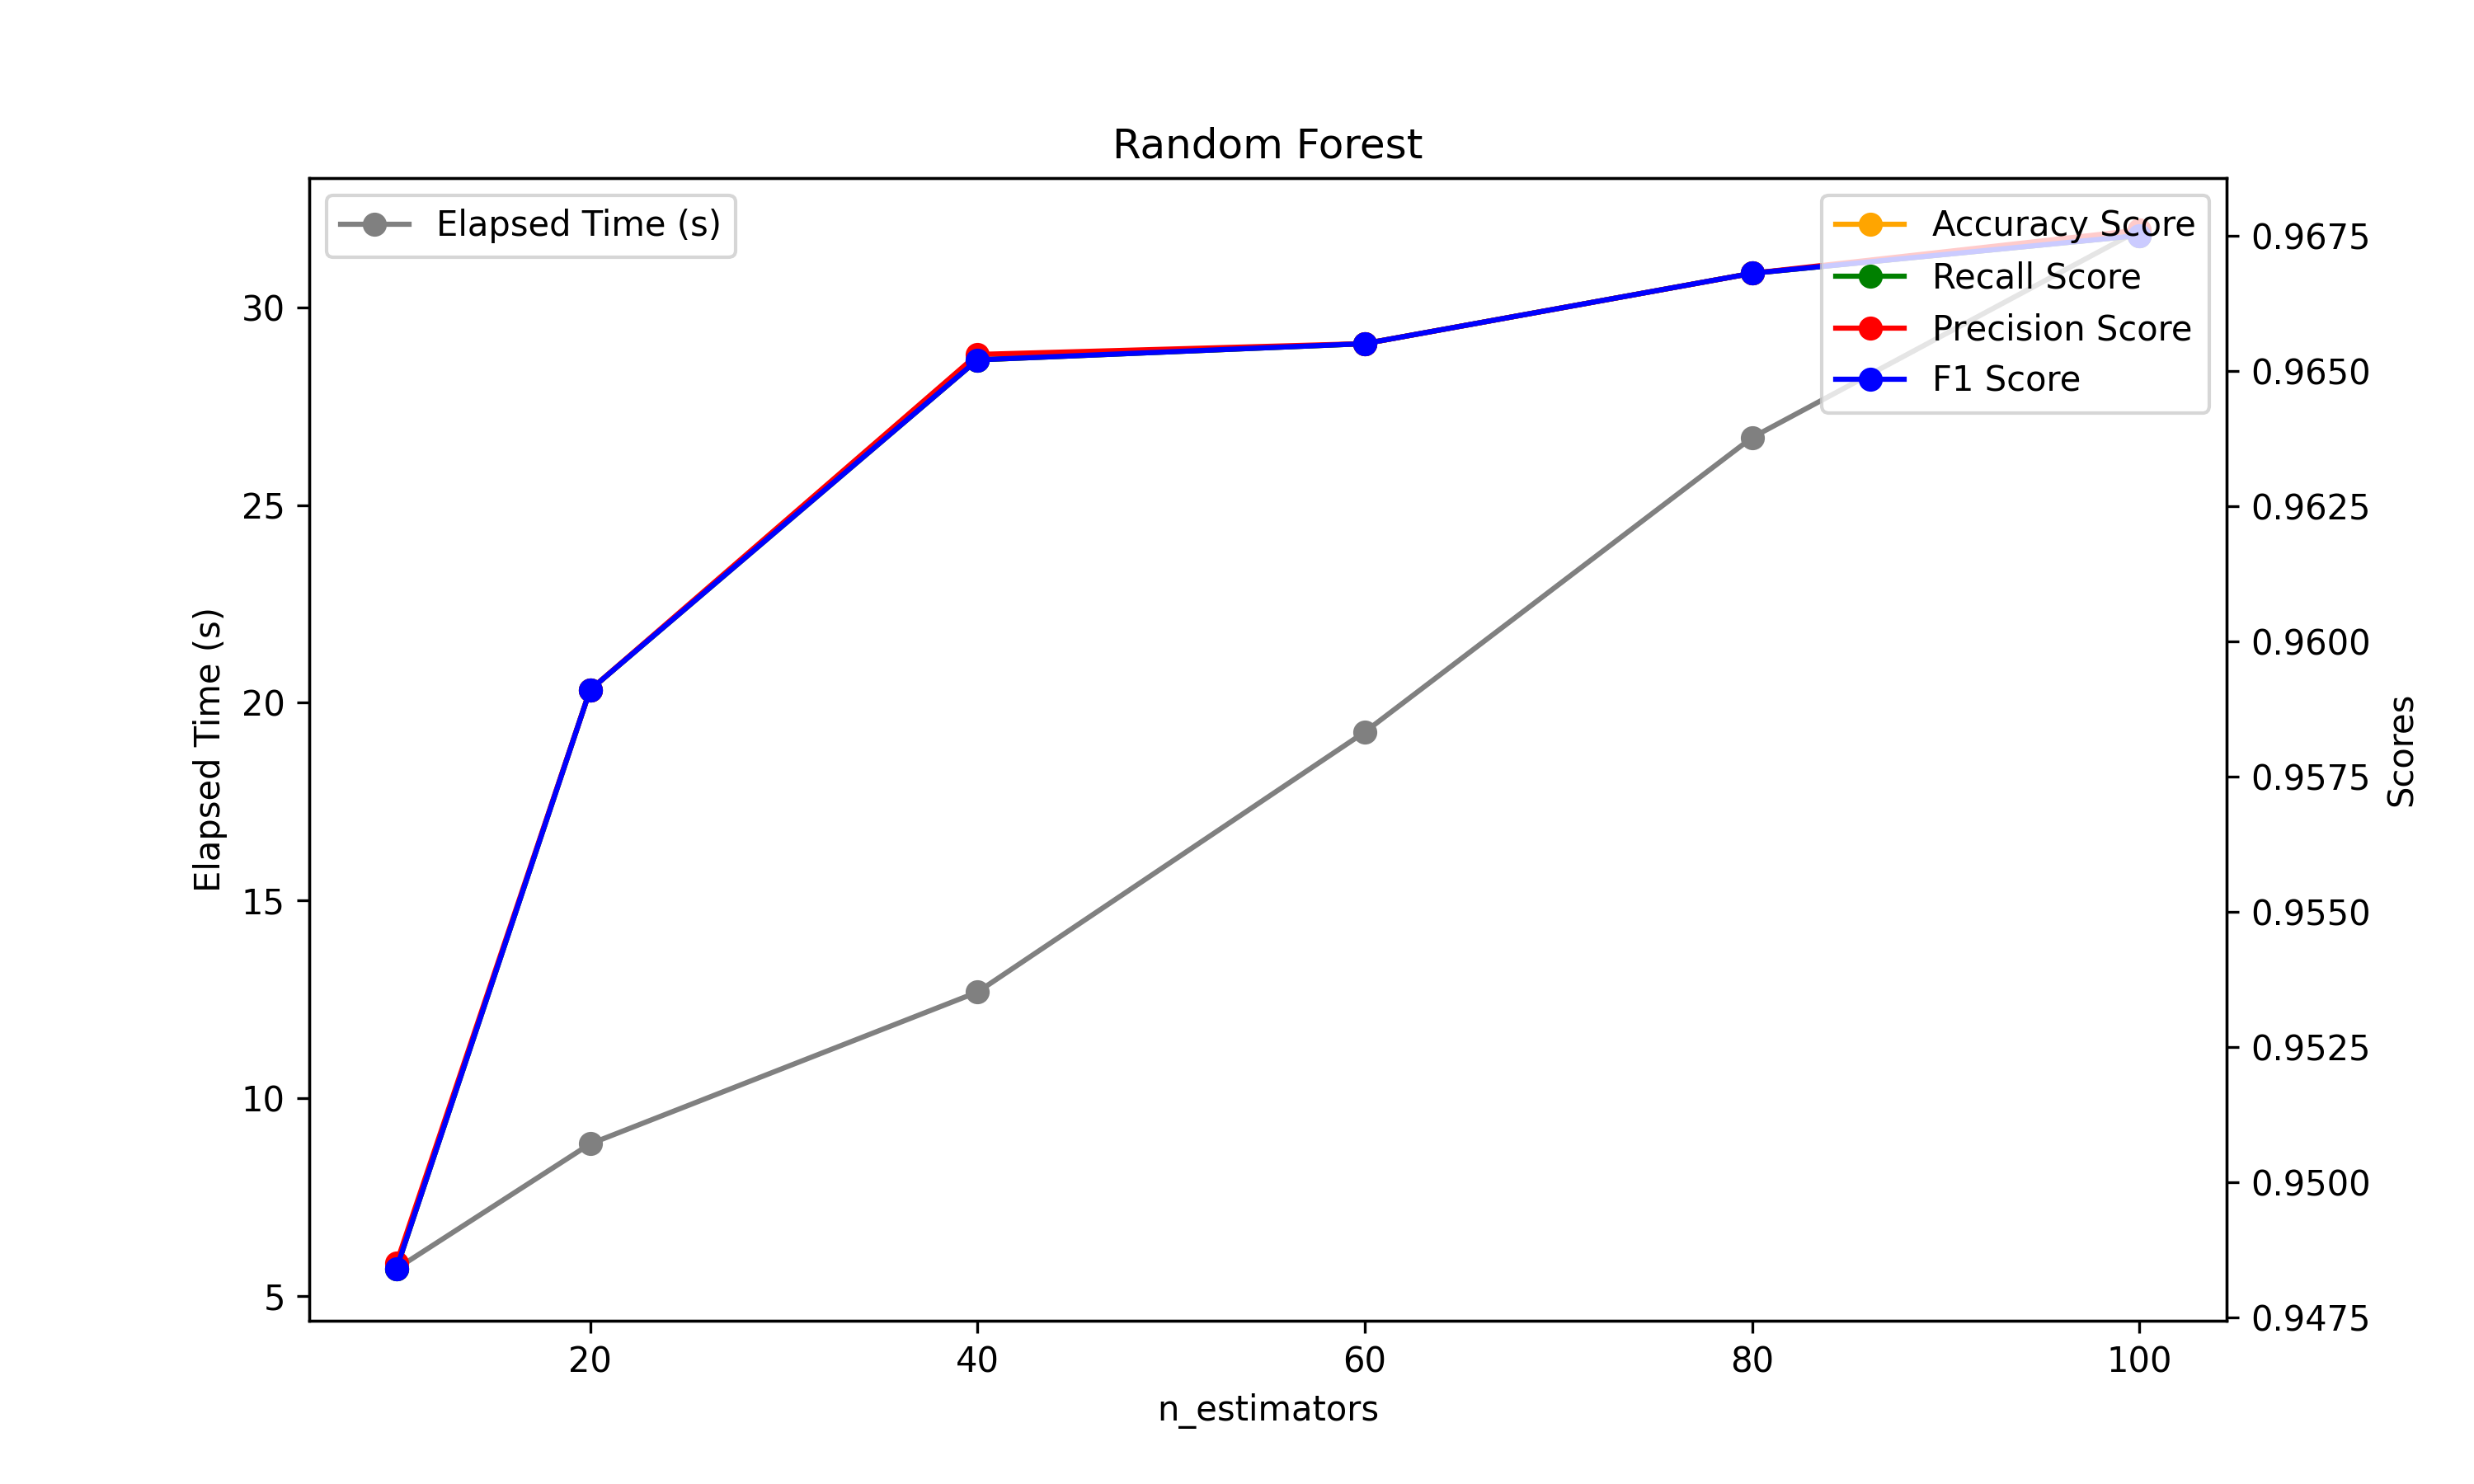
\includegraphics[scale=0.6]{pic/statistic/random_forest.png}
        \caption{Матрица ошибок Случайного леса}
        \label{ris:graph-forest}
    \end{figure}
\end{center}

Так, матрица ошибок, полученная в результате обучения модели Случайного леса, представлена на рисунке~\ref{ris:matrix-forest}.

\begin{center}
    \begin{figure}[H]
        \center{\includegraphics[width=0.4\linewidth]{image}}
        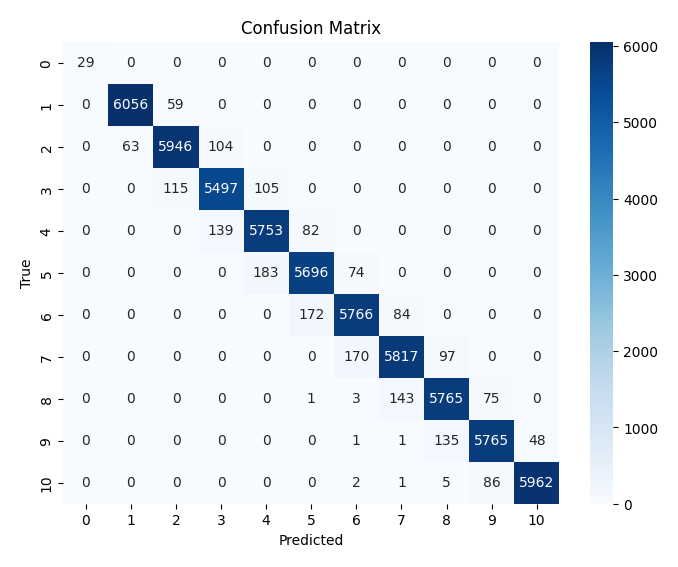
\includegraphics[scale=0.6]{pic/classification/random_forest.png}
        \caption{Матрица ошибок Случайного леса}
        \label{ris:matrix-forest}
    \end{figure}
\end{center}
\vspace{1.5em}

Результаты рассчитанных метрик для реализованных моделей классификации представлены в таблице~\ref{tabular:table-classification}.

\begin{table}[H]
    \onehalfspacing \caption{Метрики задач классификации}
    \medskip
        \begin{tabular}{|l|c|c|c|}
        \hline
            \backslashbox{}{}  & precision & recall & F-score \\ \hline
            Decision Tree & 0.9405 & 0.9406 & 0.9405 \\  \hline 
            Random Forest & 0.9675 & 0.9675 & 0.9675 \\  \hline 
            Gradient Boosting & 0.9393 & 0.9391 & 0.9389 \\  \hline 
            AdaBoosting & 0.3162 & 0.6698 & 0.2596 \\  \hline 
            Naive Bayes & 0.6258 & 0.6387 & 0.6273 \\  \hline 
        \end{tabular}
    \label{tabular:table-classification}
\end{table}

\subsection{Оценка моделей классификации с помощью метрик}
\label{sec:Metrics-regression}

\textbf{Средняя абсолютная ошибка} (Mean Absolute Error, MAE) -- это метрика, измеряющая среднее абсолютное отклонение предсказанных значений от фактических. MAE вычисляется как средняя абсолютная разница между предсказанными значениями и их соответствующими истинными значениями.

\[
MAE = \frac{1}{n}\sum_{i=1}^{n} |y_i - \hat{y}_i|
\]

\vspace{1.5em}

\textbf{Средняя квадратичная ошибка} (Mean Squared Error, MSE) -- это метрика, измеряющая среднее квадратичное отклонение предсказанных значений от фактических. MSE является средним из квадратов разностей между предсказанными значениями и их соответствующими истинными значениями.

\[
MSE = \frac{1}{n}\sum_{i=1}^{n} (y_i - \hat{y}_i)^2
\]

\vspace{1.5em}

\textbf{Коэффициент детерминации} (\( R^2 \)) -- это метрика, измеряющая долю дисперсии зависимой переменной, которая объясняется независимыми переменными в модели. \( R^2 \) принимает значения от 0 до 1 и интерпретируется как процент дисперсии зависимой переменной, который может быть объяснен моделью. Значение близкое к 1 указывает на хорошее соответствие модели данным, тогда как значение близкое к 0 означает, что модель не объясняет вариативность данных.

\[ 
R^2 = 1 - \frac{\sum_{i=1}^{n} (y_i - \hat{y}_i)^2}{\sum_{i=1}^{n} (y_i - \bar{y})^2} 
\]

где \( \bar{y} \) - среднее значение зависимой переменной. 

\vspace{1.5em}

Эти метрики являются основными инструментами для оценки качества моделей в задачах регрессии, помогая понять, насколько хорошо модель справляется с предсказанием целевых переменных.

Результаты рассчитанных метрик для реализованных моделей регрессии представлены в таблице~\ref{tabular:table-classification}.

\begin{table}[H]
    \onehalfspacing \caption{Метрики задач регрессии}
    \medskip
        \begin{tabular}{|l|c|c|c|}
        \hline
            \backslashbox{}{}  & MSE & MAE & $R^2$ \\ \hline
            Decision Tree & 9762901.26 & 466.59 & 0.2150 \\  \hline 
            Random Forest & 5496062.27 & 355.25 & 0.5580 \\  \hline 
            Gradient Boosting & 5517549.55 & 367.19 & 0.5563 \\  \hline 
            Linear Regression & 7067983.04 & 530.50 &  0.4317 \\  \hline 
        \end{tabular}
    \label{tabular:table-classification}
\end{table}